\chapter{Data sources}

\section{Identification of data sources}

\begin{challengebox}
	\textbf{How to access the data (options considered).} \\[0.25em]
To build a warehouse, we needed a reliable way to collect market listings at scale.
We considered three approaches:
\begin{enumerate}
	\item \textbf{In-game memory scanning} to read shop states directly from the game process.
	\textit{Rejected:} high risk of violating game rules and getting banned.

	\item \textbf{Classic HTML web scraping} of \url{https://metin2alerts.com/store/}.
	\textit{Rejected:} the site is paginated and the market is massive.
	At the time of writing, the market contains roughly \textbf{1697 pages} and \textbf{31122 items}.
	Scraping would be slow, brittle, and could still produce messy/incomplete data.

	\item \textbf{Client-side reverse engineering (chosen)}: observe the website network traffic to identify the real data endpoints.
	\\
		\textit{Accepted:} this approach retrieves structured JSON directly (consistent format, fast to download, and easier to validate).
\end{enumerate}

	\textbf{Outcome.} \\[0.25em]

By reverse engineering the client network requests, we discovered that the site fetches market listings from server-specific JSON snapshots and enriches them with several reference JSON files.
This discovery directly influenced the warehouse design and the ETL strategy (which fields to keep, which reference files to join, and which attributes to normalize).
\end{challengebox}

\section{Description of sources used}
The project uses three categories of sources:
\begin{itemize}
  \item \textbf{Web JSON (market snapshots)} from Metin2Alerts: server-specific listing snapshots.
  \item \textbf{Web JSON (static reference)} from Metin2Alerts: dictionaries and metadata needed to interpret the listings.
  \item \textbf{PostgreSQL warehouse}: the structured analytical store (facts, dimensions, aggregates).
\end{itemize}

\section{Type of data}
\begin{itemize}
  \item Semi-structured data: JSON (market listings and reference files).
  \item Structured data: PostgreSQL tables (facts, dimensions, aggregates, views).
\end{itemize}

Once we decided that client-side reverse engineering was the safest and most scalable acquisition method, the next question was:
	\textit{ what exactly does the website download, and how are the files connected?}

By observing the network traffic of \url{https://metin2alerts.com/store/}, we found that the website relies on:
\begin{itemize}
  \item \textbf{Market snapshots}: large JSON arrays containing the actual listings for a given server.
  \item \textbf{Reference files}: smaller JSON files that provide meaning and labels (names, bonus/stat meanings, UI strings, etc.).
\end{itemize}

\begin{figure}[H]
    \centering
    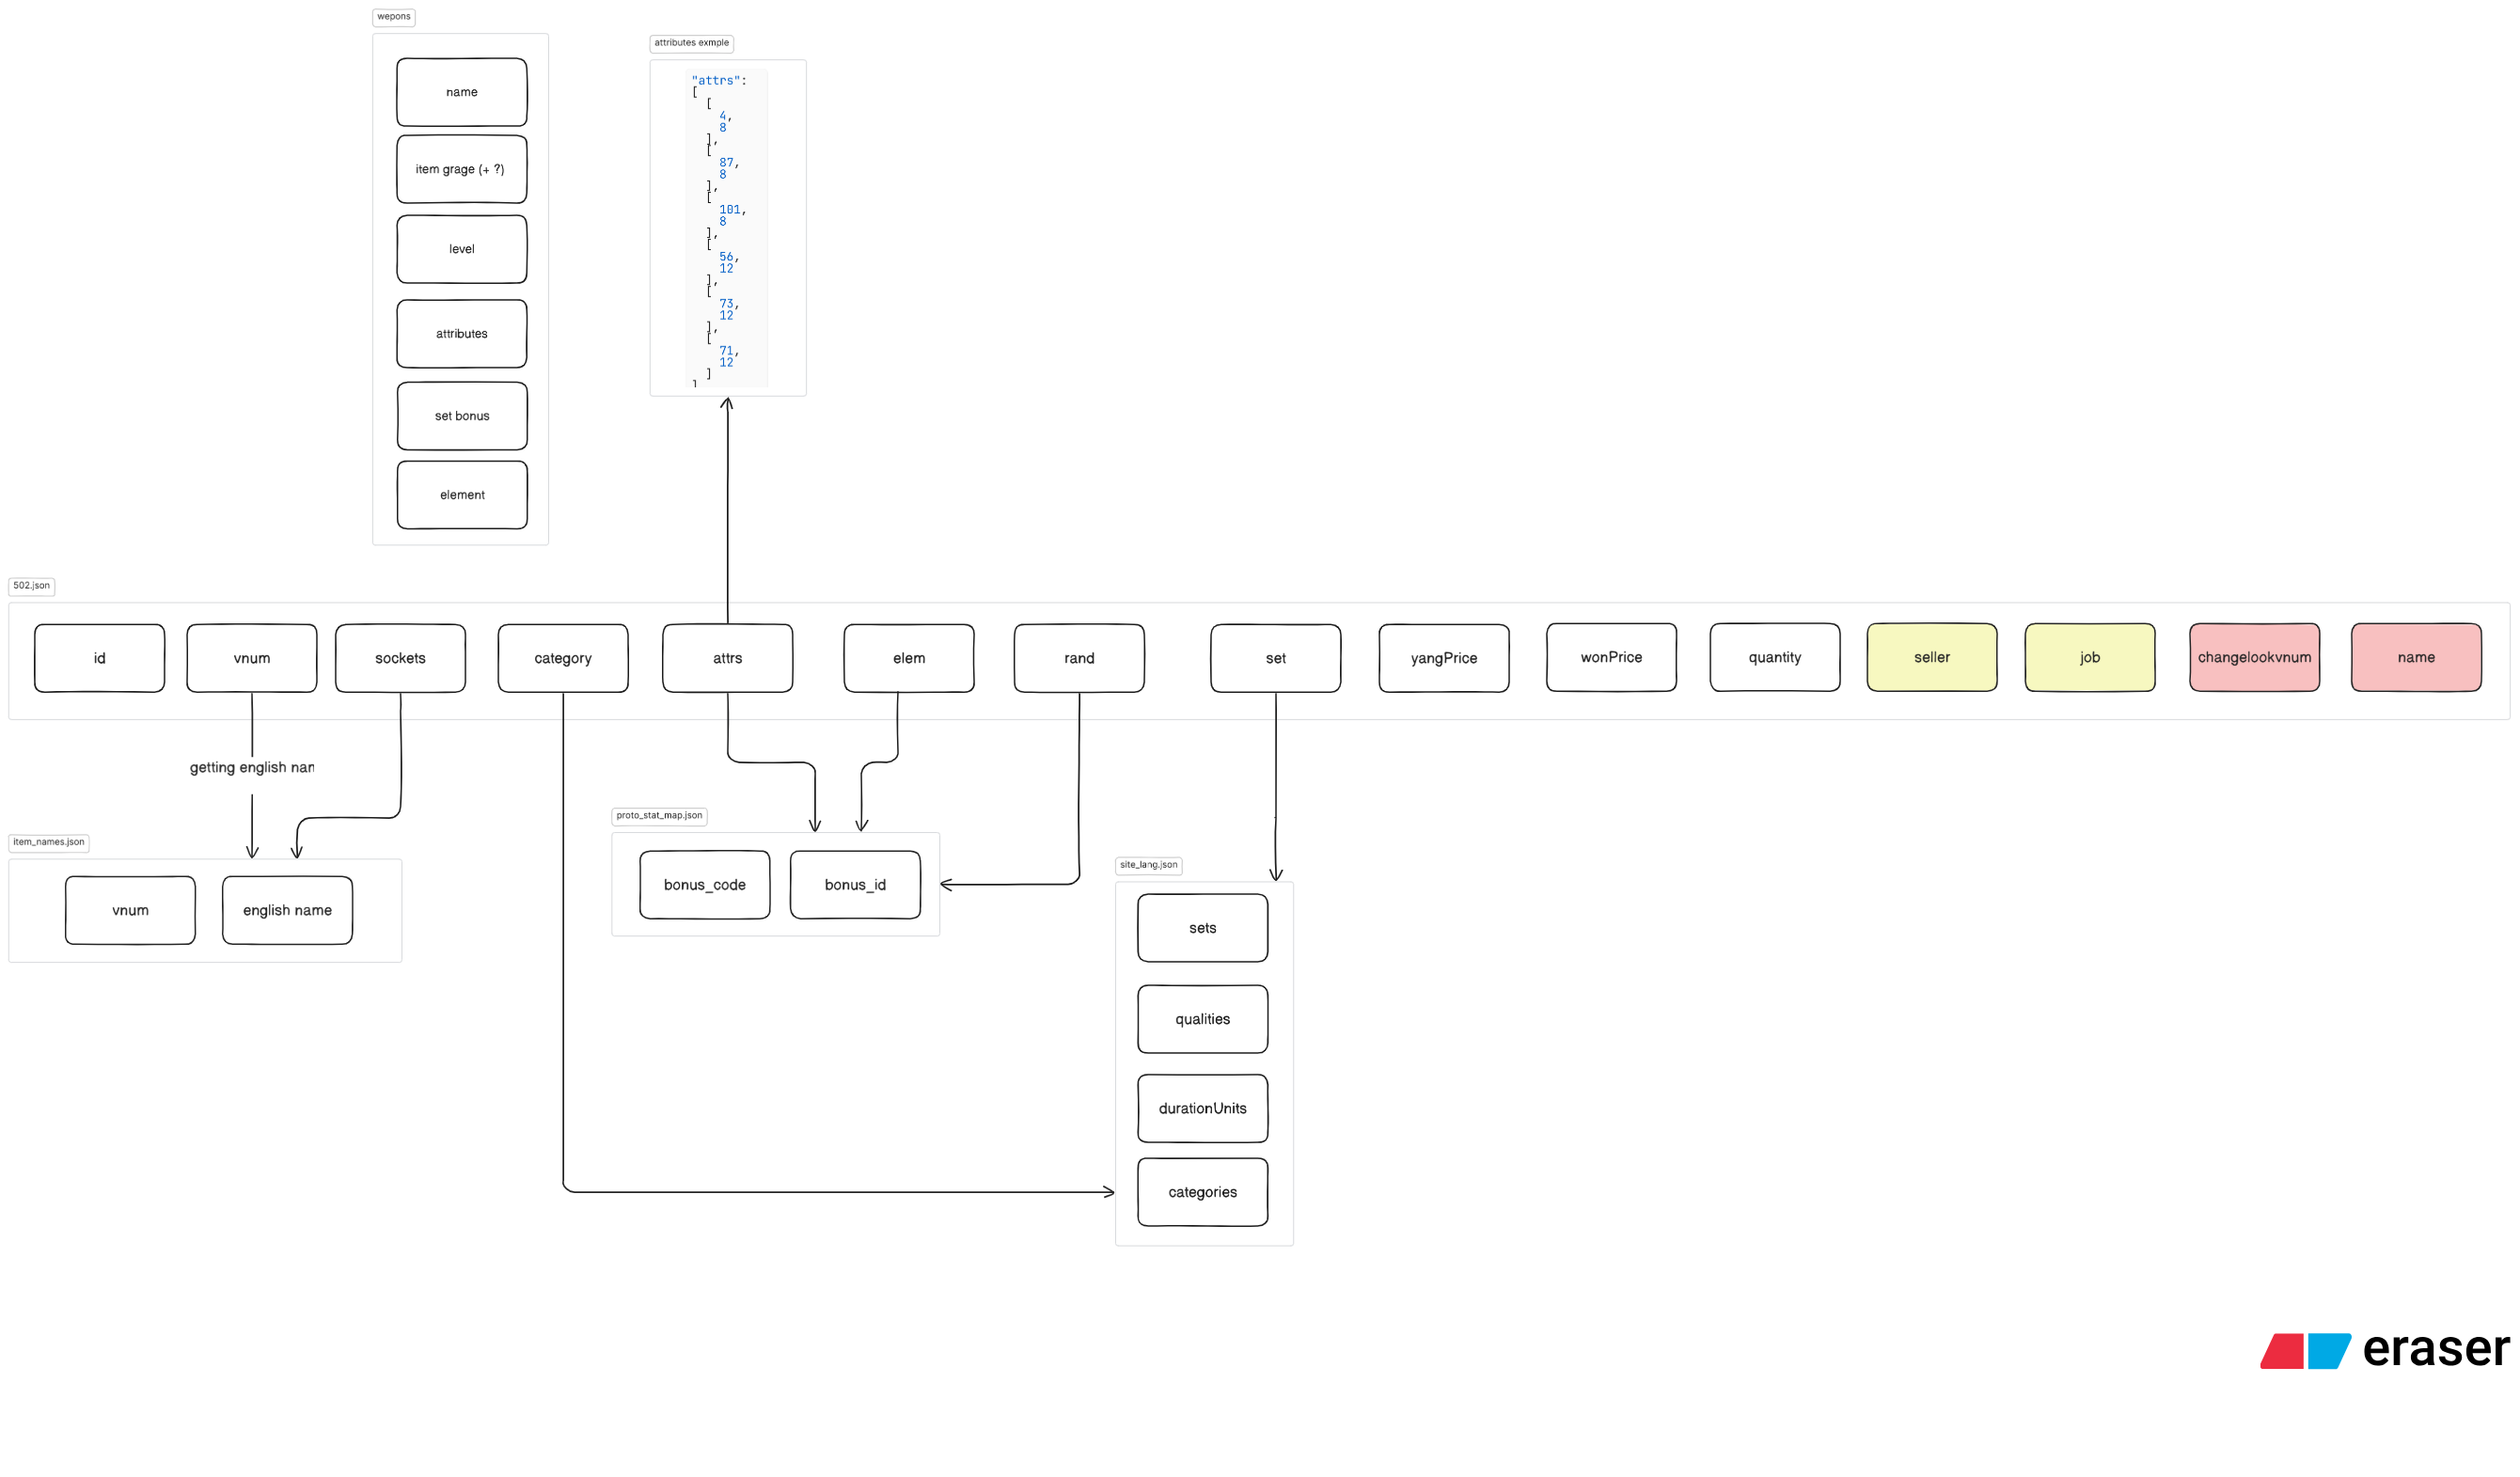
\includegraphics[width=0.92\linewidth]{filesRs.png}
    \caption{Relationships Between Market JSON and Reference JSON Files}
    \label{fig:json-relationships}
\end{figure}


\section{Discovered JSON files and their roles}
\subsection{Market data (large, server-specific)}
The website fetches market listings as a JSON snapshot per server:
\begin{itemize}
  \item \texttt{https://metin2alerts.com/store/public/data/502.json} (Europe)
  \item \texttt{https://metin2alerts.com/store/public/data/71.json} (Teutonia)
\end{itemize}
Each file contains a large array of listings, where each listing includes identity fields (like \texttt{vnum}), seller information, prices, and detailed item attributes.

\subsection{Static reference files (small, meaning/labels)}
The website also relies on several reference JSON files (English in our project) to interpret the listing payload.
We synchronize these files once and reuse them throughout the ETL:

\begin{table}[!ht]
\centering
\caption{Reference JSON files used to interpret listings}
\begin{tabularx}{\linewidth}{@{}lX@{}}
	\toprule
	\textbf{File} & \textbf{Purpose (observed)} \\
\midrule
	\texttt{/m2\_data/en/stat\_map.json} & Human-readable mapping for a subset of game stats/labels.
\\
	\texttt{/m2\_data/proto\_stat\_map.json} & Maps stat/bonus identifiers to their meaning (used to interpret \texttt{attrs}, \texttt{rand}, and \texttt{elem}).
\\
	\texttt{/m2\_data/item\_proto.json} & Base item metadata (type/subtype and proto fields that help decode weapon/armor stats).
\\
	\texttt{/m2\_data/en/item\_names.json} & Stable English item names indexed by \texttt{vnum} (used to avoid localization issues).
\\
	\texttt{/m2\_data/item\_icon.json} & Maps items to icon filenames for UI/display.
\\
	\texttt{/m2\_data/en/itemdesc.json} & Item descriptions (textual reference).
\\
	\texttt{/m2\_data/en/site\_lang.json} & UI strings and enumerations (including labels for special ``set'' titles).
\\
	\texttt{/m2\_data/en/mob\_names.json} & Monster names (auxiliary reference).
\\
	\texttt{/m2\_data/en/pet\_skills.json} & Pet skills reference (auxiliary reference).
\\
\bottomrule
\end{tabularx}
\end{table}

\section{Reverse engineered listing fields (market payload)}
After collecting the snapshot JSON, we still needed to interpret the meaning of the fields.
The following mapping summarizes the key fields used by the ETL.

\begin{longtable}{@{}p{0.22\linewidth}p{0.73\linewidth}@{}}
\caption{Market listing fields and interpreted semantics}\label{tab:market-payload-fields}\\
		\toprule
		\textbf{Field} & \textbf{Meaning and usage in the warehouse} \\
\midrule
\endfirsthead
		\toprule
		\textbf{Field} & \textbf{Meaning and usage in the warehouse} \\
\midrule
\endhead
\bottomrule
\endfoot

	\texttt{vnum} & \textbf{Virtual number}: the item identifier. All items with the same base identity share the same \texttt{vnum}. Used as the natural key for \texttt{dim\_item}. \\

	\texttt{name} & The displayed name in the market payload (often localized, e.g., German). \textbf{Ignored for analysis labels}; we use English mapping from \texttt{item\_names.json}. \\

	\texttt{seller} & Seller name (listing context). Stored in fact tables for analysis (seller behavior, clustering, etc.). \\

	\texttt{yangPrice} & Price in \textbf{Yang} (small denomination). Stored as \texttt{transaction\_price\_yang}. \\

	\texttt{wonPrice} & Price in \textbf{Won} (large denomination). Stored as \texttt{transaction\_price\_won}. \\

	\texttt{quantity} & Quantity listed. Meaningful mainly for stackable items; for non-stackable items it is typically 1. \\

	\texttt{job} & A class/job identifier associated with the listing context. Stored as \texttt{job\_id} for server-level and class-level filtering. \\

	\texttt{attrs} & Attributes (bonuses) array. Each element is a pair \texttt{[bonus\_id, bonus\_value]}. These are normalized into up to 7 attribute slots in \texttt{fact\_item\_attributes}. \\

	\texttt{sockets} & Array of socketed stones (typically stone \texttt{vnum}s). Stored to allow filtering and valuation heuristics. \\

	\texttt{rand} & Random bonus list (same structure as \texttt{attrs}), commonly observed on higher-level items. Treated as attributes but marked internally as random when needed. \\

	\texttt{set} & Special set/title flag (one of a finite set of possibilities). Labels are derived from \texttt{site\_lang.json}. \\

	\texttt{elem} & Element info. Observed structure: \texttt{[elem\_bonus\_id, primary\_values, secondary\_values]}. In practice we keep the primary list and compute the total power as the sum of its values; the secondary list is ignored for our KPIs. The element bonus id meaning is taken from \texttt{proto\_stat\_map.json}. \\

	\texttt{changelookvnum} & Appearance override: if non-zero, the item is visually changed to another \texttt{vnum}. Useful for UI and some filtering logic. \\

\end{longtable}

\section{Why the correlations matter}
The warehouse design and ETL steps depend directly on these correlations:
\begin{itemize}
  \item \textbf{Stable naming}: \texttt{vnum} from the market snapshot must be joined with \texttt{item\_names.json} to obtain a consistent English label.
  \item \textbf{Bonus semantics}: \texttt{attrs/rand/elem} only become meaningful after mapping IDs using \texttt{proto\_stat\_map.json}.
  \item \textbf{Type-aware parsing}: base item type/subtype and proto values from \texttt{item\_proto.json} influence how we interpret weapon/armor stats and which facts/dimensions are populated.
\end{itemize}
Because of this dependency chain, we treat reference files as first-class sources and synchronize them before processing market snapshots.

\begin{riskbox}
\textbf{Data quality issues encountered and mitigations:}
\begin{itemize}
  \item \textbf{Localization / inconsistent item names}: market payload may include localized names. 
  Mitigation: enforce English naming via synced reference mapping (vnum $\rightarrow$ name).

  \item \textbf{Schema uncertainty}: attribute arrays, sockets, and nested fields vary by item type. 
  Mitigation: reverse engineer and normalize into stable columns (e.g., 7 attribute slots) and computed metrics.

  \item \textbf{Duplicates}: exact replicas may appear multiple times in one snapshot. 
  Mitigation: deduplicate identical listings before loading.

  \item \textbf{Temporal bias}: snapshots represent the market at fetch time. Some listings may persist across time. 
  Mitigation: use a time dimension and batch timestamps to track snapshots consistently.
\end{itemize}
\end{riskbox}

\placeholderfigure{Example Market JSON Structure (annotated)}{0.92\linewidth}{5.5cm}

